% ==========================================================
% =                         ANEXOS                         =
% ==========================================================
%\phantomsection
\section{OLDatasets} \label{appendix:OLDatasets}

Standing for OpenLABEL Datasets, OLDatasets is a custom parser from NuImages format to OpenLABEL format developed in order to integrate it with the \aclink{VCD} library ecosystem developed and maintained by Vicomtech \footnote{\url{https://www.vicomtech.org/en/}}.

\begin{table}[h]
    \centering
    \begin{tabular}{l c c c c}
        \toprule
        \textbf{Name} & \textbf{ID} & \textbf{trainId} & \textbf{Dynamic} & \textbf{Color (RGB)} \\
        \midrule
        background                          & 0  & 0  & False & (0, 0, 0) \\
        animal                              & 1  & 1  & True  & (255, 0, 0) \\
        human.pedestrian.adult              & 2  & 2  & True  & (220, 20, 60) \\
        human.pedestrian.child              & 3  & 3  & True  & (220, 20, 60) \\
        human.pedestrian.construction\_worker & 4  & 4  & True  & (220, 20, 60) \\
        human.pedestrian.personal\_mobility & 5  & 5  & True  & (220, 20, 60) \\
        human.pedestrian.police\_officer    & 6  & 6  & True  & (220, 20, 60) \\
        human.pedestrian.stroller           & 7  & 7  & True  & (220, 20, 60) \\
        human.pedestrian.wheelchair         & 8  & 8  & True  & (220, 20, 60) \\
        movable\_object.barrier             & 9  & 9  & False & (190, 153, 153) \\
        movable\_object.debris              & 10 & 10 & False & (152, 251, 152) \\
        movable\_object.pushable\_pullable  & 11 & 11 & False & (255, 0, 0) \\
        movable\_object.trafficcone         & 12 & 12 & True  & (111, 74, 0) \\
        static\_object.bicycle\_rack        & 13 & 13 & False & (255, 0, 0) \\
        vehicle.bicycle                     & 14 & 14 & True  & (119, 11, 32) \\
        vehicle.bus.bendy                   & 15 & 15 & True  & (0, 60, 100) \\
        vehicle.bus.rigid                   & 16 & 16 & True  & (0, 60, 100) \\
        vehicle.car                         & 17 & 17 & True  & (0, 0, 142) \\
        vehicle.construction                & 18 & 18 & True  & (255, 0, 0) \\
        vehicle.emergency.ambulance         & 19 & 19 & True  & (255, 0, 0) \\
        vehicle.emergency.police            & 20 & 20 & True  & (255, 0, 0) \\
        vehicle.motorcycle                  & 21 & 21 & True  & (0, 0, 230) \\
        vehicle.trailer                     & 22 & 22 & True  & (0, 0, 110) \\
        vehicle.truck                       & 23 & 23 & True  & (0, 0, 70) \\
        vehicle.ego                         & 24 & 24 & True  & (255, 255, 255) \\
        flat.driveable\_surface             & 25 & 25 & False & (128, 64, 128) \\
        \midrule
        ignore                              & 255 & 255 &       &        \\
        \bottomrule
    \end{tabular}
    \caption{Semantic labels defined for NuImages masks}
    \label{tab:semantic_labels}
\end{table}

\begin{figure}[h!]
    \centering
    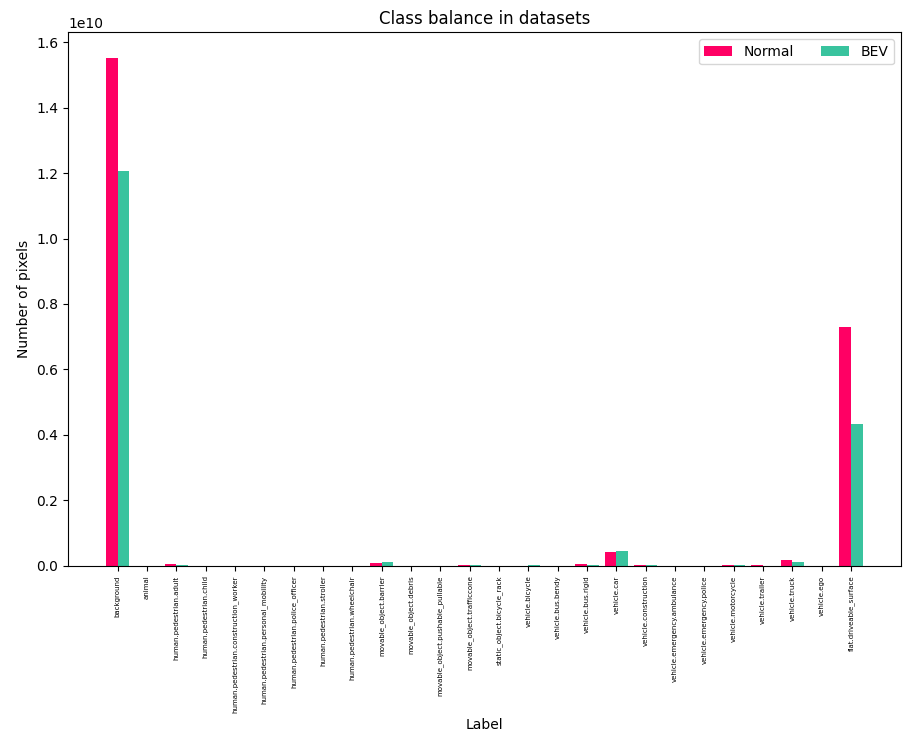
\includegraphics[width=\linewidth]{images/appendix/dataset_class_balance_pixels.png}
    \caption{Number of pixels per class in datasets}
    \label{fig:dataset_class_balance_pixels}
\end{figure}

\begin{figure}[h!]
    \centering
    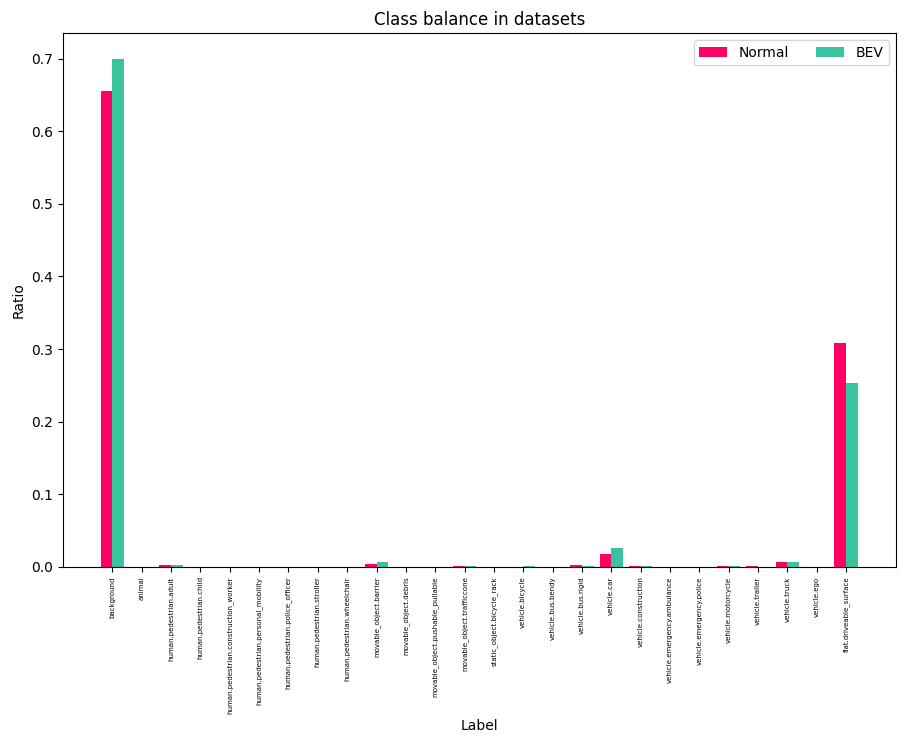
\includegraphics[width=\linewidth]{images/appendix/dataset_class_balance_ratio.png}
    \caption{Relative distribution of classes in dataset}
    \label{fig:dataset_class_balance_ratio}
\end{figure}

\section{Rotation matrix to euler angles}
Here \cite{euler_from_matrix} is the pseudocode.


\section{Color palette}
\begin{table}[h]
    \centering
    \renewcommand{\arraystretch}{1.5} % Increase row height
    \setlength{\tabcolsep}{12pt} % Increase column spacing
    \begin{tabular}{c c}
        \toprule
        \textbf{Hex Code} & \textbf{Color Sample} \\
        \midrule


        \#FF0064 & \cellcolor[HTML]{FF0064} \hspace{2cm} \\
        \#FF62A0 & \cellcolor[HTML]{FF62A0} \hspace{2cm} \\
        \#0277BD & \cellcolor[HTML]{0277BD} \hspace{2cm} \\
        \#2AB0D2 & \cellcolor[HTML]{2AB0D2} \hspace{2cm} \\
        \#7700A0 & \cellcolor[HTML]{7700A0} \hspace{2cm} \\
        \#B200EF & \cellcolor[HTML]{B200EF} \hspace{2cm} \\
        \#00A032 & \cellcolor[HTML]{00A032} \hspace{2cm} \\
        \#03FF52 & \cellcolor[HTML]{03FF52} \hspace{2cm} \\
        \#FF9800 & \cellcolor[HTML]{FF9800} \hspace{2cm} \\
        \#FFB03B & \cellcolor[HTML]{FFB03B} \hspace{2cm} \\

        % \#F44336 & \cellcolor[HTML]{F44336} \hspace{2cm} \\
        % \#EF5350 & \cellcolor[HTML]{EF5350} \hspace{2cm} \\
        % \#F1464E & \cellcolor[HTML]{F1464E} \hspace{2cm} \\
        % \#FF9800 & \cellcolor[HTML]{FF9800} \hspace{2cm} \\
        % \#FF0064 & \cellcolor[HTML]{FF0064} \hspace{2cm} \\
        % \midrule
        % \#4CAF50 & \cellcolor[HTML]{4CAF50} \hspace{2cm} \\
        % \#86BB48 & \cellcolor[HTML]{86BB48} \hspace{2cm} \\
        % \#39C39E & \cellcolor[HTML]{39C39E} \hspace{2cm} \\
        % \midrule
        % \#0277BD & \cellcolor[HTML]{0277BD} \hspace{2cm} \\
        % \#0097A7 & \cellcolor[HTML]{0097A7} \hspace{2cm} \\
        % \#2AB0D2 & \cellcolor[HTML]{2AB0D2} \hspace{2cm} \\
        % \#01A1FF & \cellcolor[HTML]{01A1FF} \hspace{2cm} \\
        % \#0073B7 & \cellcolor[HTML]{0073B7} \hspace{2cm} \\
        \bottomrule
    \end{tabular}
    \caption{Color Palette}
    \label{tab:color_palette}
\end{table}
